\capitulo{3}{Conceptos teóricos}
\section{Geoposicionamiento}

El geoposicionamiento es la capacidad de determinar o estimar la posición geográfica de un objeto\cite{GeoPosicionamiento}. Este concepto es fundamental en el proyecto, ya que lo utilizamos para calcular las localizaciones \textit{indoor}.

Para entender en profundidad el proyecto creado, es necesario conocer algunos conceptos que están relacionados con el geoposicionamiento:

\begin{itemize}
    \item \textit{\textbf{GPS}}: Sistema que permite la localización de un objeto sobre la tierra con precisión de hasta centímetros.\cite{wiki:gps}
    \item \textbf{Triangulación}: En el contexto de \textit{GPS} y mediante satélites que mandan señales. Con tres satélites, consiste en averiguar el ángulo de las tres señales respecto al punto de medición. Con esto se consigue la posición relativa respecto a los tres satélites.
    \item \textbf{Localización indoor}: Surge del margen de error de las mediciones \textit{GPS} y se trata de obtener la localización de un usuario dentro de un edificio mediante triangulación. Se replica este sistema a menor escala con distintas placas \textit{UWB} posicionadas de manera que se pueda conseguir la posición relativa de una de ellas respecto a las otras.
\end{itemize}


\section{Interfaz de programación de aplicaciones (API)}
Este concepto sirve para conectar componentes y que se puedan comunicar entre ellos, como por ejemplo una aplicación web y una base de datos.

Se utiliza la arquitectura \textit{Restful}, eso significa que se ha implementado utilizando estos principios \textit{REST}\cite{apiRest}:
\begin{itemize}
    \item \textbf{Sin estado}: La \textit{API} trata a todas las peticiones entrantes por igual, y no guarda información de ninguna de ellas.
    \item \textbf{Operaciones Especificas}: Cada operación es concreta y especifica, no multifuncional.
    \item \textbf{Sintaxis estandarizada}: Cada recurso es accesible únicamente mediante su identificador de recursos uniforme (\textit{URI}), que es el enlace de acceso a un recurso.
    \item \textbf{Cliente-Servidor}: Se utiliza una arquitectura cliente servidor para hacer las peticiones, siendo el servidor el que tiene la lógica de los recursos y los expone al cliente.
En la figura 3.1 se expone la interacción entre la \textit{API}, el cliente y la base de datos
\end{itemize}
\begin{figure}[h]
    \centering
    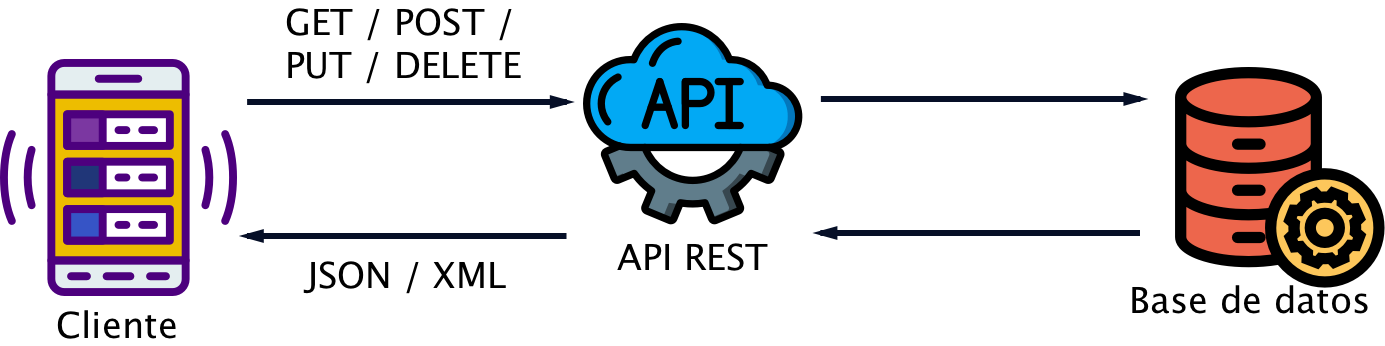
\includegraphics[width=10cm,height=10cm,keepaspectratio]{img/Esquema API.png}
    \caption{Ilustración de conexiones de una \textit{API Rest} \cite{EsquemaAPI}.}
    \label{fig:example_GPS}
\end{figure}
\FloatBarrier
Todos estos conceptos, además, se han desarrollado utilizando el estándar \textit{OpenAPI 3.0} con la ayuda de \textit{Swagger Editor}. 

\textit{OpenAPI} se utiliza para la definición de los componentes de una \textit{API} mediante un archivo de extensión .yaml.
Mediante ese archivo y con la ayuda de la herramienta \textit{Swagger Editor}, se genera un proyecto en \textit{Python} y \textit{Flask} listo para conectar con la base de datos e implementar los métodos de los \textit{endpoints}, que son puntos finales en un canal de comunicación.






\section{Sesiones de usuario}
Para el desarrollo del proyecto, se decidió que los usuarios no iban a tener cuentas de usuario, sino que que se iba a trabajar con sesiones especiales para las pruebas  de la manera más realista.

A un usuario no le interesa tener una cuenta en un museo que seguramente solo vaya a visitar un par de veces, por lo que las sesiones eran la mejor opción. Las sesiones tienen las siguientes características:
\begin{itemize}
    \item Una sesión de usuario en la base de datos, se creará cuando un usuario introduzca en el formulario de Login un alias y el id de su \textit{Tag} asignado.
    \item Cuando un usuario termina la sesión del tour, la fila con su alias no se borra, solo se desenlaza la \textit{Tag}, así más adelante, si otro usuario introduce el mismo alias se reutilizará la sesión.
    \item Si un usuario introduce un alias que está siendo utilizado, no permitirá el enlace con el \textit{Tag}, así que se tendrá que elegir otro alias.
\end{itemize}

\section{Intercambio de Recursos de Origen Cruzado (CORS)}
Este concepto se implementa en las navegadores como medida de seguridad, para las peticiones \textit{HTTP} que se ejecutan.\cite{amazon:CORS}

El uso de \textit{CORS} se utiliza en las cabeceras de las peticiones \textit{HTTP}, para que el servidor las acepte, teniendo que poner distintas cabeceras extra para el correcto funcionamiento de la política, que son:

\begin{itemize}
    \item \textit{\textbf{mode: 'cors'}}: esto implementa el modo \textit{cors} en la petición, no es parte de la cabecera, pero es necesario para indicar el tipo de petición que se quiere utilizar desde el navegador.
    \item \textit{\textbf{Access-Control-Allow-Origin}}: Esta cabecera indica si los recursos pueden ser compartidos con el origen. En el proyecto se utiliza el elemento '*' (wildcard) que indica que no es necesario el uso de credenciales en el servidor.
    \item \textit{\textbf{Access-Control-Allow-Methods}}: Esta cabecera indica los métodos aceptados cuando se accede a un recurso.
    \item \textit{\textbf{Access-Control-Allow-Headers}}: Esta cabecera indica los encabezados que pueden ser utilizados en la petición.
\end{itemize}

Para poder utilizar los endpoints de la \textit{API} se tuvo que encapsular la \textit{API} con una librería llamada \textit{flask-cors}, permitiendo que acepte peticiones con \textit{CORS} que vengan desde los navegadores.
\begin{figure}[b]
    \centering
    \includegraphics[width=10cm,height=10cm,keepaspectratio]{img/GPS-satélites.jpg}
    \caption{Ilustración de la triangulación \textit{GPS} \cite{TringulacionGPS}.}
    \label{fig:example_GPS}
\end{figure}
Esto da una capa extra de seguridad en las peticiones, ya que permite bloquear peticiones potencialmente peligrosas. En el proyecto práctico del TFG realmente no se necesita esa capa extra de seguridad, ya que es un proyecto de investigación, por lo que se ha implementado de la manera más básica posible para simplemente permitir todas las peticiones desde los navegadores.

\section{Localización Indoor}
En esta sección se van a explicar los conceptos correspondientes a la implementación de la localización \textit{indoor}, incluida la representación de las coordenada locales en el mapa.

Para calcular la localización general de un usuario normalmente se utiliza
la tecnologia \textit{GPS}, utilizándose para geolocalizar usuarios en cualquier
punto de la tierra con una precisión de metros, mediante el uso de señales,
triangulando la posición con satélites, como se muestra en la figura 3.2. Sin embargo, en ciertos entornos,
como por ejemplo dentro de un edificio, la señal puede no llegar, haciendo
que no sea posible aplicar la tecnologia \textit{GPS} para la localización \textit{indoor}. 

\begin{figure}[b]
    \centering
    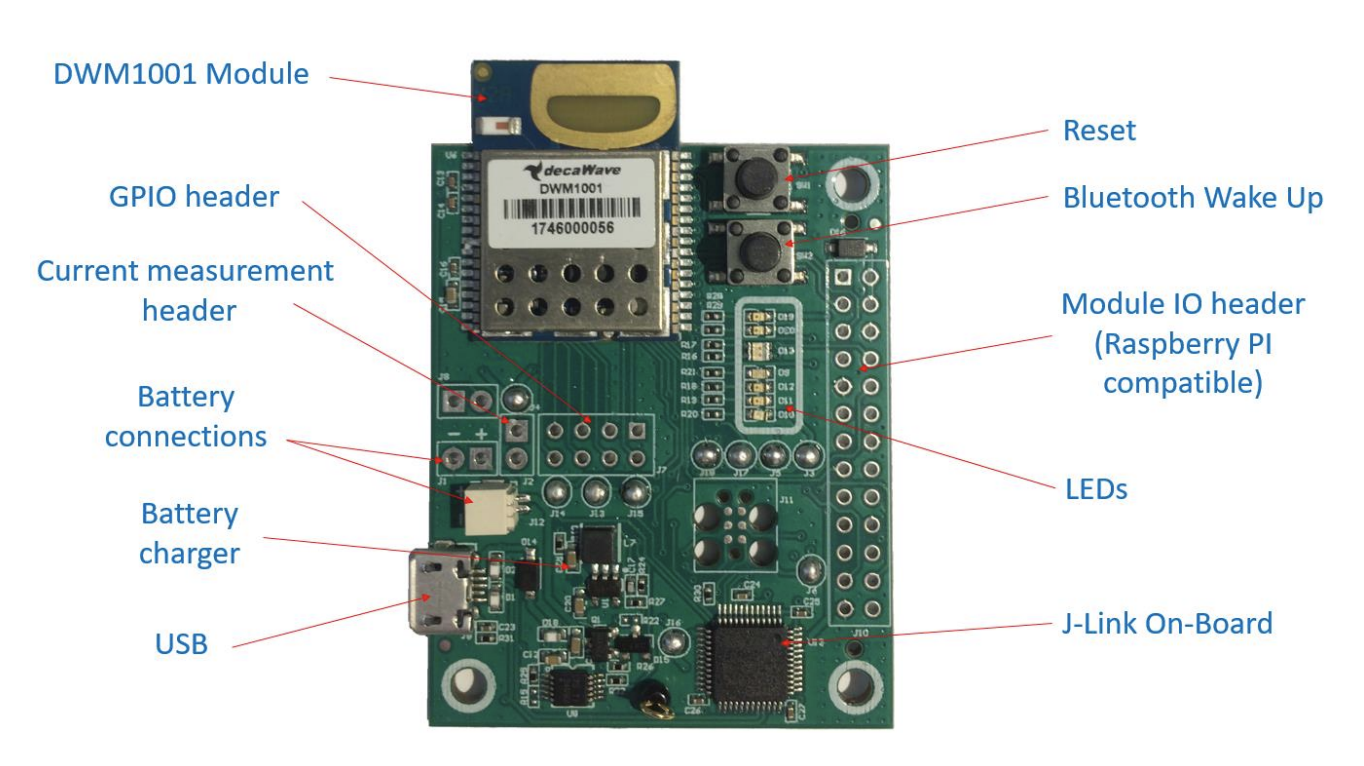
\includegraphics[width=10cm,height=10cm,keepaspectratio]{img/MDEK1001.png}
    \caption{Placa \textit{UWB} MDEK1001 utilizada en este proyecto.}
    \label{fig:example_board}
\end{figure}

De manera general, existen pocas soluciones de localización \textit{indoor} producidas por la investigación a gran escala de estos sistemas, produciendo datos
no tan fiables como los esperados. Haciendo que las soluciones propuestas
hasta el momento, \textit{Wifi} o \textit{Bluetooth Low Energy (BLE)}, no alcancen los
objetivos mínimos necesarios para su implementación en interiores.

\textit{UWB} es el acrónimo de \textit{Ultra Wide Band}, banda ultra ancha, tecnología que utiliza un ancho de banda mayor a 500 MHz\cite{xataka:uwb}. Esta es la tecnología elegida para implementar la geolocalización indoor mediante la triangulación.

El modelo de las placas \textit{UWB} es el \textbf{MDEK1001} usando en el proyecto un total 12 placas, 6 con el rol de \textit{anchors} para consultas pasivas, 2 placas con el rol de \textit{listener}, y 4 con el rol de \textit{tags} como usuarios que triangulan su posición respecto a los demás anchors, trabaja a una frecuencia de 2.4 GHz y tienen una tasa de refresco de 10 Hz.

En la figura 3.3 podemos ver una placa \textit{UWB} modelo \textit{MDEK1001}, con sus distintas partes.


\begin{figure}[t]
    \centering
    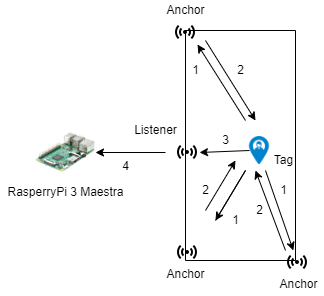
\includegraphics[width=10cm,height=10cm,keepaspectratio]{img/Esquema Conexiones UWB.drawio.png}
    \caption{Esquema de conexiones básico para \textit{localización indoor} en el proyecto.}
    \label{fig:exmaple_indoor_loc}
\end{figure}

Todo este entorno permite trabajar sobre placas \textit{Raspberries Pi 3}, que es un ordenador integrado a modo de placa, como punto de salida con la \textit{API} de cada habitación implementada. La comunicación entre placas \textit{UWB} y \textit{Raspberry} se hace mediante una de las placas, que tiene el rol de \textit{listener}.

Las \textit{Raspberries} funcionan con una arquitectura maestro esclavo y sirven para unificar una red de conexión entre las placas y poder comunicarse con la \textit{API} actualizando la información en el base de datos.

Como las pruebas son con dos entornos pequeños, se han utilizado dos \textit{Raspberries} maestras que se encargan de interactuar con la \textit{API} y las placas \textit{UWB} se mantienen conectadas por la poca distancia que existe entre ellas.

Un ejemplo de triangulación de \textit{UWB} se encuentra en la figura 3.4, donde podemos ver un \textit{Tag} calculado su posición en la representación local respecto a los \textit{anchors} y comunicándoselo al \textit{listener} para que la \textit{Raspberry} mueva esos datos al sistema.





Las \textit{Raspberries} maestras también se encargan de hacer la conversión de la representación local al tipo de datos que pueda utilizar el mapa para representar los elementos.

Esta conversión se hace mediante la traslación del eje de coordenadas X e Y a otro eje Latitud y Longitud. Teniendo las dimensiones de la sala reales en metros, y las coordenadas aproximadas de tres puntos coincidiendo con esquinas de la una sala rectángulo, colocando un \textit{anchor} en cada esquina, convenientemente posicionamos uno de los \textit{anchor} como centro de coordenadas de los ejes X e Y, junto con el ángulo que forman los distintos ejes, mediante trigonometría podemos hacer la traslación de un punto, obteniendo su latitud y longitud reales en el mapa. 

\begin{figure}[t]
    \centering
    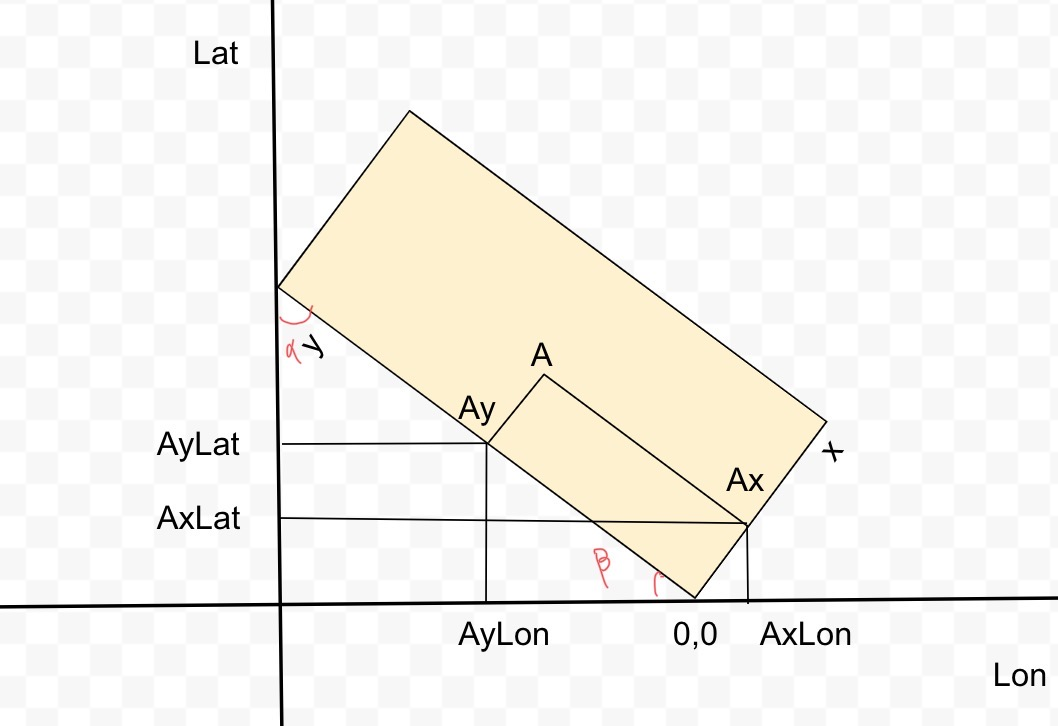
\includegraphics[width=10cm,height=10cm,keepaspectratio]{img/traslation_coorinates.jpg}
    \caption{Conversión de las coordenadas X
e Y a los ejes de Latitud y de Longitud.}
    \label{fig:traslation_coordinates}
\end{figure}


En la figura 3.5 podemos ver como el punto A se proyecta sobre el eje de coordenadas de Latitud y Longitud, teniendo dos puntos sobre estos nuevos ejes del punto principal.


Después, y sabiendo que 1 metro en el mapa equivalen a 120000 metros, que es la escala que utilizamos en el mapa, podemos crear una fórmula general de como hacer la traslación de un punto entre ejes de coordenadas:


\[ diffLat = \frac{Y*sin(ángulo) + X*sin(90 ^{\circ}  + ángulo)}{120000} \]
\[ diffLon = \frac{Y*cos(ángulo) + X*cos(90^{\circ} + ángulo)}{120000} \]

Simplificando queda:



\[ diffLat = \frac{Y*sin(ángulo) + X*cos(ángulo)}{120000} \]
\[ diffLon = \frac{Y*cos(ángulo) + X*sin(ángulo)}{120000} \]

Teniendo en cuenta que el centro de coordenadas de X e Y se tiene como 0,0 y su representación en Latitud y Longitud, el cálculo final de las coordenadas del punto quedaría:

\[ Lat = centerLat + diffLat \]

\[ Lon = centerLon + diffLon  \]

La formula general quedaría:

\[ Lat = centerLat + \frac{Y*sin(ángulo) + X*cos(ángulo)}{120000} \]

\[ Lon = centerLon + \frac{Y*cos(ángulo) + X*sin(ángulo)}{120000}  \]

Una vez calculadas las coordenadas, se implementará una llamada a un \textit{endpoint} para la persisitencia o modificado de las coordenadas en la base de datos.


\section{Geofencing}

El \textit{geofencing} es el proceso de intersecar las coordenadas de uno o más polígonos con las coordenadas de uno o más puntos, dándonos métricas importantes sobre el posicionamiento de los puntos.

Este proceso se puede realizar a tiempo real, y entonces obtenemos cuándo los puntos en movimiento entran a los polígonos estáticos, siendo los polígonos las salas y los puntos los usuarios, creamos el concepto de cuando un usuario entra a una sala y con esto podemos:

\begin{itemize}
    \item Saber en qué sala está un usuario a tiempo real.
    \item Saber cuántos usuarios hay en una sala a tiempo real.
\end{itemize}

En la figura 3.6 podemos ver como un \textit{Tag} se encuentra dentro de una \textit{Room}, por lo que se le puede aplicar \textit{geofencing} para obtener el nombre de la \textit{Room} en la que se encuentra.

\begin{figure}[t]
    \centering
    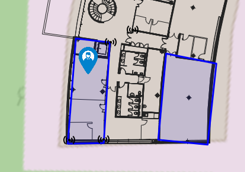
\includegraphics[width=10cm,height=10cm,keepaspectratio]{img/geofencing.png}
    \caption{Sistema de \textit{Geofencing}. Las posición del visitante se interseca con los límites de la \textit{Room} (en azul).}
    \label{fig:traslation_coordinates}
\end{figure}
